
\subsection{Machine Analysis}
We use the random forest algorithm to predict program outcome and fault type. A random forest is essentially an ensemble of single decision trees, as illustrated in ~\ref{fig:rf} \cite{breiman2001random}. It captures different models of the data, with each decision tree representing a model, and allows us to analyze the importance of different features. 

\begin{figure}[t]
\begin{center}
   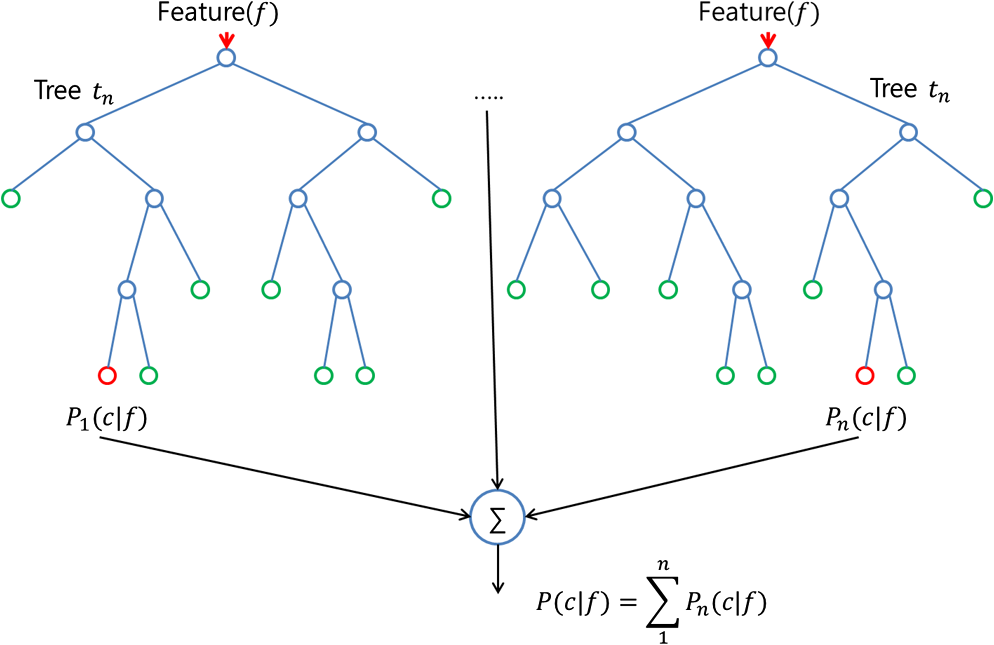
\includegraphics[width=0.95\linewidth]{./figures/rf.png}
\end{center}
   \caption{}
\label{fig:rf}
\end{figure}

\subsubsection{Training and Testing}
We randomly select $60\%$ of instances for training and $40\%$ of instances for testing. Our dataset consists of $98,000$ data instance.